%!TEX root = ./Intro_to_CC.tex

\section{Problem 3: Hydronium cation}
\label{sec:problemIII}
\subsection*{Planar hydronium cation}

This exercise covers how to perform geometry optimizations.
Specifically, we will relax the \ch{H3O^+} molecule starting from an initial planar guess for the geometry. 

\begin{enumerate}

  \item The planar \ch{H3O+} geometry has been provided in the file \Verb{geom_planar.xyz}.
  \begin{gaussinput}[title=Contents of \Verb{geom_planar.xyz}]
O    0.00    0.00   0.00
H    0.92   -0.53   0.00
H   -0.92   -0.53   0.00
H    0.00    1.06   0.00

  \end{gaussinput}
  
  \item Create an \Verb{input.com} file, using the template provided in the first problem. 
  Use the \Verb{HF} level of theory and the \Verb{6-31G(d,p)} basis set. 
  We want to relax the geometry and perform the vibrational analysis of the ion. 
  Therefore, replace the \Verb{sp} keyword (`single-point') from the template with \Verb{opt freq} (`optimization' and `frequency'). 
  After removing the information for the previous molecule, add the geometry of the cation at the end of the input file\sidenote{copy by hand or, in the terminal, type \bashinline{cat geom_planar.xyz >> input.com} to append the contents to then end of the file}.
  
  \item Run Gaussian.
  \begin{bashinput}
      g16 input.com &
  \end{bashinput} 
  
  \item Once the calculation is complete, visualize the results, we will use the notebook in JupyterLab. 
  Execute the first few cells of the section until you get an output that shows you the molecule. 
  This cell also outputs the total energy of the ion. 
  Note the command that outputs this value. 
  Also note that the molecule only shows bonds to two of the hydrogen atoms. 
  What does the fully relaxed structure look like? 
  Do you think that this is the structure of \ch{H3O+} in the gas phase? 
  % Save a picture of the ion.
  
  \item   We'll use two additional cells to define bonds between the oxygen and all three hydrogens and to reformat the vibrational information so we can visualize it. 
  The final cells in this section of the notebook will show the corrected structure and list the normal modes/vibrations with their IR intensity, sorted by wavenumber (\si{\wn}). 
  Click through the spectrum to animate some of the vibrations. 
  You can select all of the vibrations by clicking the menu icon \( (\vdots) \) in the upper right corner of the output view window and using the dropdown menu for ``Normal Mode''. 
  You should see that one of the frequencies is negative -- select the normal mode to which it corresponds. 
  In the discussion section (at the end of the notebook), include this table and indicate what kind of molecular motion each vibration corresponds to. 

\end{enumerate}


\subsection*{Pyramidal hydronium cation}

Next, repeat the calculations for a pyramidal hydronium cation: 
\begin{gaussinput}[title=Contents of \Verb{geom_pyramidal.xyz}]
O    0.00   0.00   0.00 
H    0.92  -0.53  -0.66 
H   -0.92  -0.53  -0.66 
H    0.00   1.06  -0.66 

\end{gaussinput}
Visualize the results again using the steps from the previous section. 
You should see the \ch{H3O+} in a pyramidal conformation now.  
Note again the total energy of the ion and compare it with the planar structure in your discussion. 
Which conformation has lower energy? 
Next, view the vibrations table and spectrum. 
If calculations were done properly, all vibrations should have positive wavenumbers. 
Describe again in the discussion section the motion the vibrations correspond to. 


\subsection*{Potential-Energy Surface Scan}

In the final problem, we are going to inspect the potential-energy surface of the hydronium ion along its umbrella mode. In the planar cation problem, you have seen that the negative\sidenote{In fact, it is imaginary, \iu{} is dropped by convention} frequency corresponds to such an `umbrella' mode. 

\begin{itemize}
  \item In a terminal window, change to the \Verb{PES} directory. 
  You will an template input file already prepared. 
  If you open it, you should see that the \( xyz \)-cartesian coordinates have been replaced with a \( z \)-matrix. 
  The \( z \)-matrix allows precise control of the geometry within single calculations.

    \begin{gaussinput}[title=\(z\)-matrix in the PES input file]
O   	                       
X   1 a                   
H   1 a   2 HOX            
H   1 a   2 HOX   3  120.0 
H   1 a   2 HOX   3 -120.0 

a=OH 
HOX= 135. -1. 45 

    \end{gaussinput}
  
  
  \item The first column shows the bonding, second shows the angles between atoms and the third column specifies the dihedral angle. 
  X is a dummy (non-existent) atom that enables control of the umbrella motion. 
  \Cref{fig:internal_coords} explains the \( z \)-matrix graphically. 
  First, calculate the \ch{O-H} distance using the functions defined in the first cell of this section and the optimized pyramidal geometry from the previous section. Replace the \Verb{OH}\sidenote{On the line that says \Verb{a=OH}} in the input file with this value. 
  Next, run the calculations using Gaussian. 
  The calculations will perform a scan along the \ch{X-O-H} angle, performing a single point calculations every \ang{1} from \SIrange{135}{90}{\degree}. 
  When the calculations are finished, import the results to Jupyter and plot the resulting potential-energy surface. 
  Discuss these results in your report.  
  The PES for angles below \ang{90} is the mirror image. Use \si{\kcal\per\mol} instead of \si{\hartree} in the report. 
  
  \begin{marginfigure}[-12\baselineskip]
    \centering
      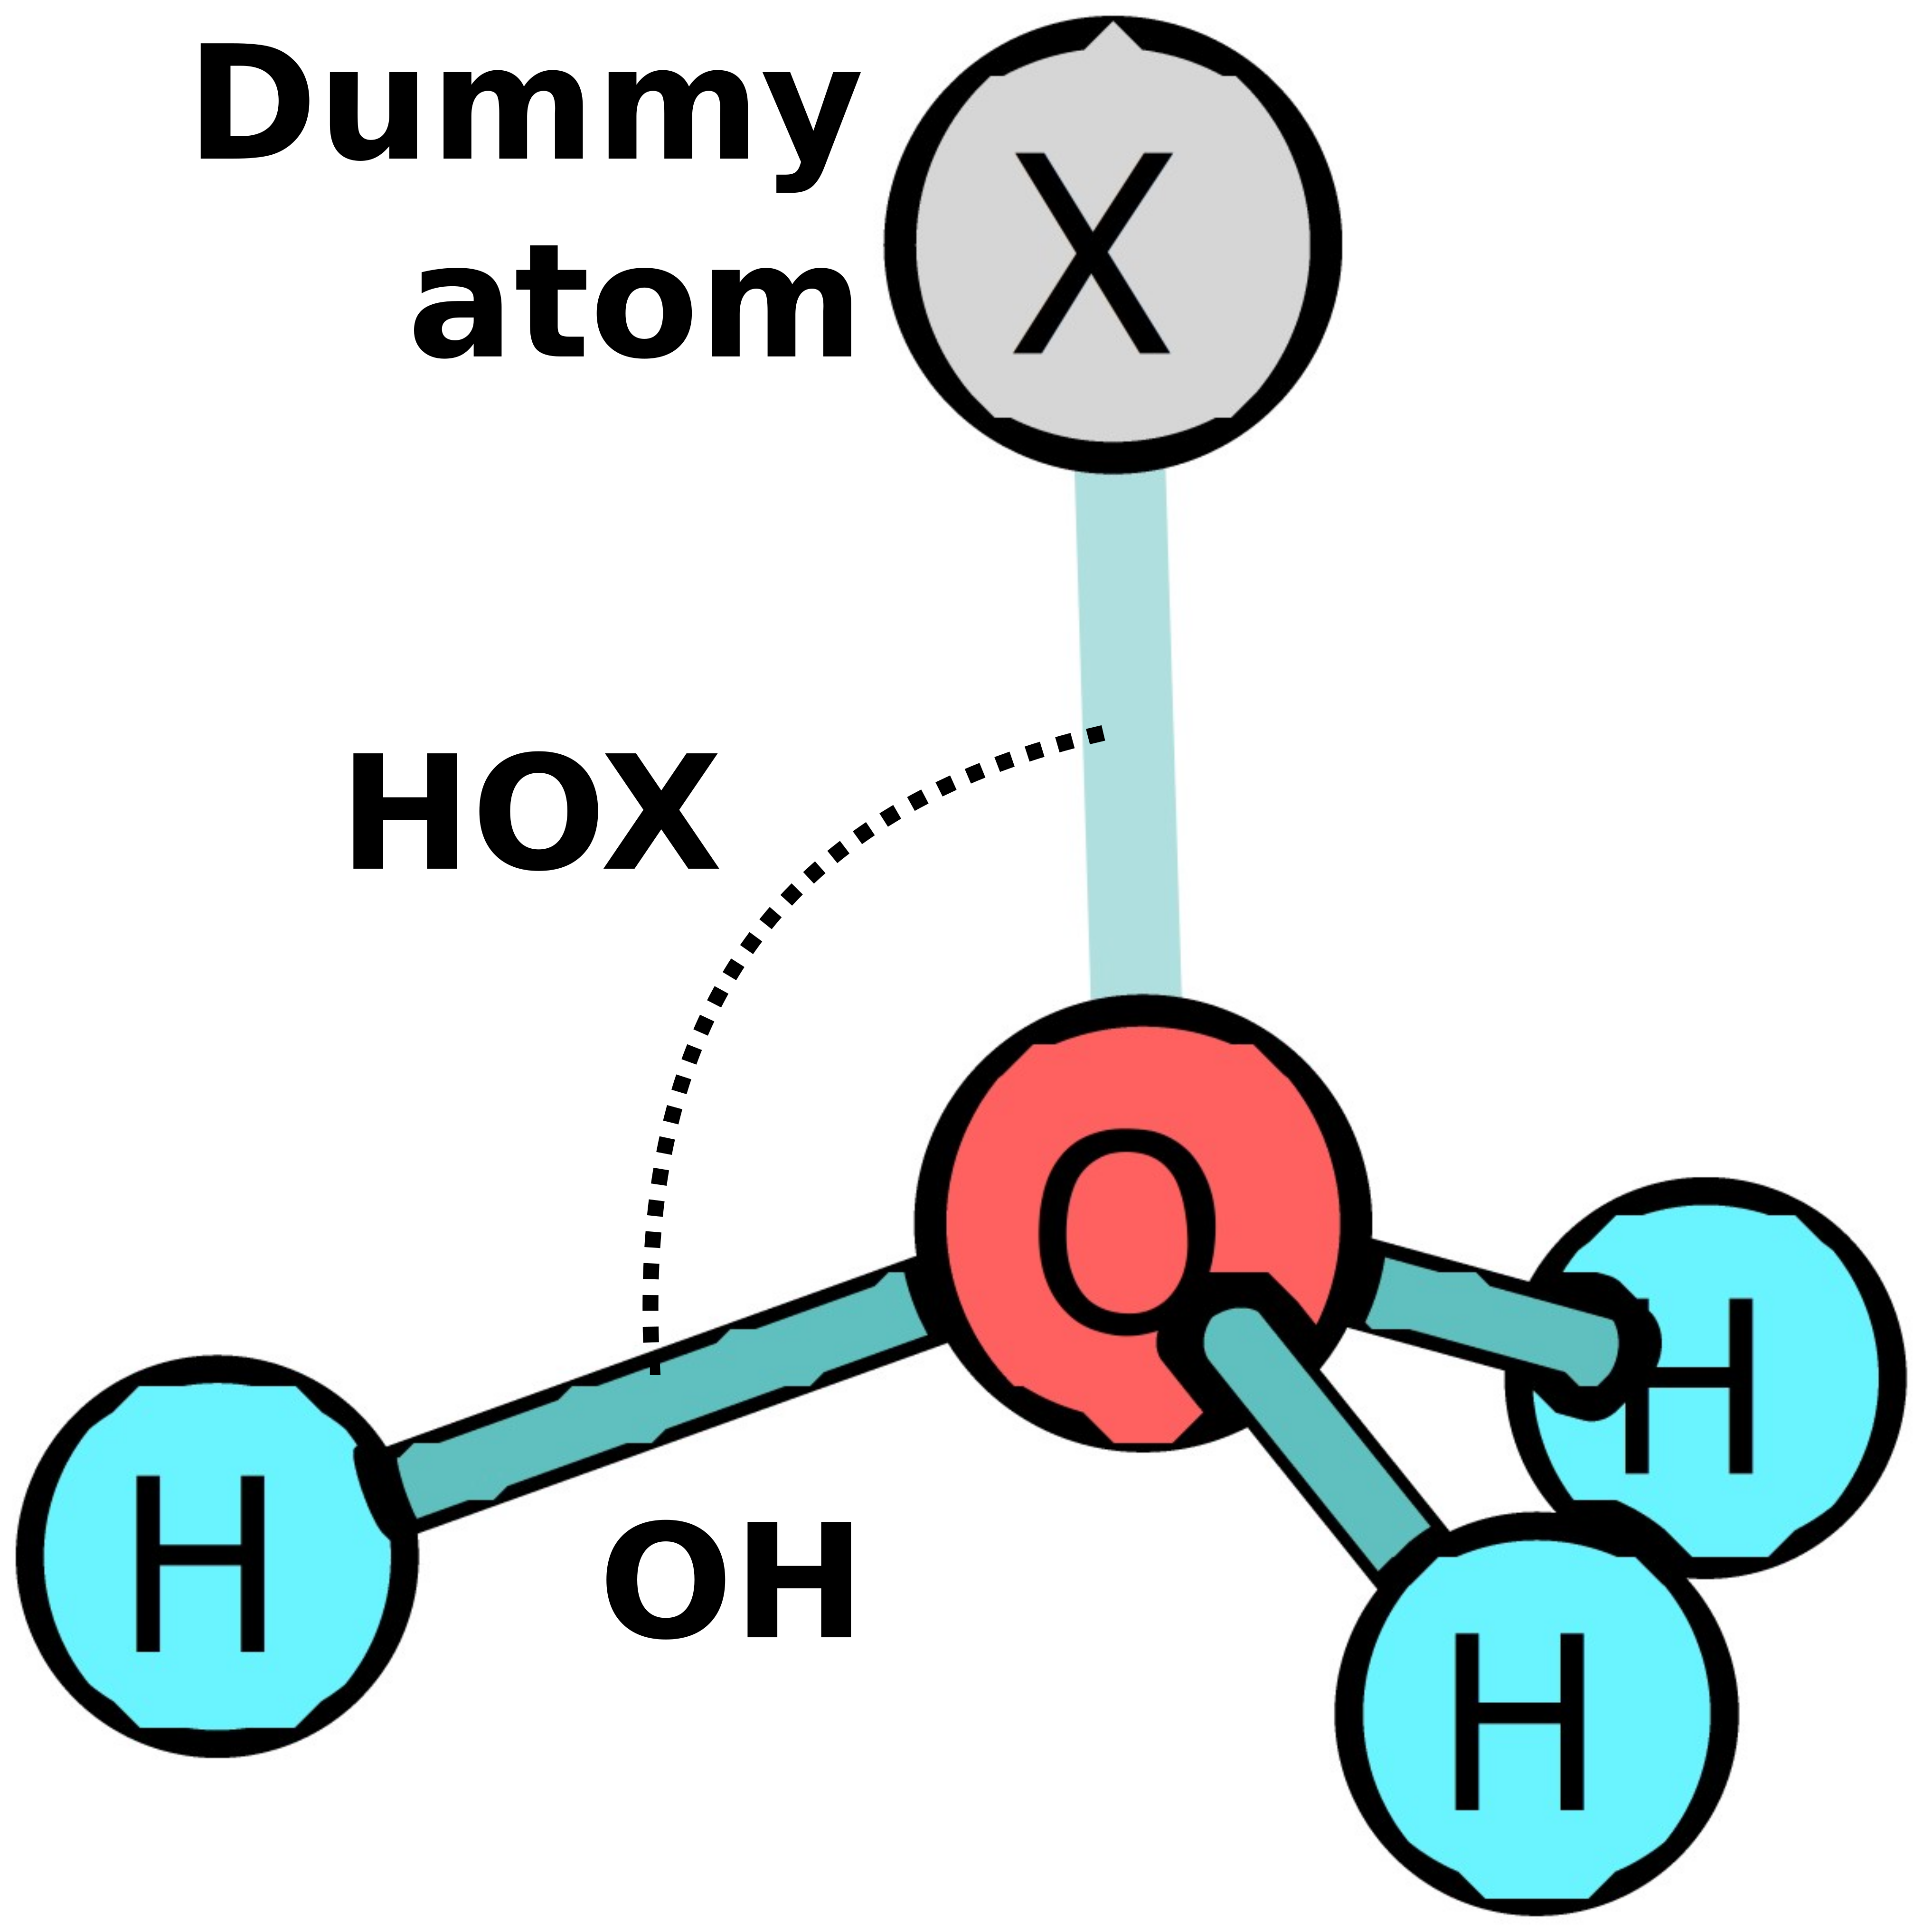
\includegraphics[width=0.75\textwidth]{pics/zmat.png}
    \caption{Definition of hydronium ion internal coordinates. 
      The calculations perform a scan along the \ch{X-O-H} coordinates for all three hydrogens from \SIrange{135}{90}{\degree}. 
      The \ang{120} dihedral angle indicates the relative position of hydrogen atoms.}
    \label{fig:internal_coords}
  \end{marginfigure}

  \item Localize the lowest-energy and transition structure along the PES and calculate the reaction barrier of the internal flip of the hydronium ion. 
  Whereas the energy of the pyramidal ion is comparable with the minimum on the PES, the energy of the optimized planar cation and the local maximum on the PES is different. 
  Why? Compare the geometries. 

  \item In the final step, rerun the calculations using the \texttt{MP2} method and compare your results. 
  You'll need to rerun the geometry optimization (for the pyramidal molecule) using the MP2 level of theory so you get the right bond length to run the PES scan of the umbrella mode. 
  Try plotting both PES scan curves in one plot to compare methods. 
  Look at the difference in final energies and the difference in the barrier energy for the two methods. 


\end{itemize}

\section*{Lab report}

For the lab report, please prepare following data.\sidenote{This is the bare minimum; there are couple of open questions in the text that you should try to assess.}
All of this can be done in the Discussion section of the Jupyter notebook. 
When you are finished, export the finished document as a PDF file  by clicking \menu{File>Export Notebook As…>Export Notebook to PDF} and email that PDF to me. 

\begin{enumerate}
  \item Plot the Total Energy vs. number of basis functions for a hydrogen atom for all methods used in Problem 1. 

  \item Plot the binding curves for HF using Hartree-Fock and PBE1PBE methods. Find the minimum distance and compute the atomization energy. 
  Plot the dipole moment as a function of the bond distance. 
  Plot both methods in the same image. You can do this with the \Verb{plt.plot()} method from the Matplotlib library. 
  If you made the distances into the index for your dataframe, you can call those values with \Verb{df.index.values}. 
  Multiple sets of \emph{x-y} data can be plotted with \Verb{plt.plot(x1, y1, x2, y2)}, where \Verb{x1}, ... are the various lists of \emph{x} and \emph{y} data. 

  \item Prepare tables listing molecular vibrations in a hydronium ion in planar and pyramidal geometries. 
  Make sure the wavenumbers are shown for all molecular vibrations. 

  \item Plot the PES along the HOX coordinate using HF and MP2 methods. 
  Use \si{\kcal\per\mol} for the \( y \)-axis. 
  Compute the heigh of the barrier separating two pyramidal structures (the energy required to pass over the planar intermediate on the PES). 
  
\end{enumerate}


